% Options for packages loaded elsewhere
\PassOptionsToPackage{unicode}{hyperref}
\PassOptionsToPackage{hyphens}{url}
\PassOptionsToPackage{dvipsnames,svgnames,x11names}{xcolor}
%
\documentclass[
  0.875em,
  letterpaper,
  DIV=11,
  numbers=noendperiod]{scrartcl}

\usepackage{amsmath,amssymb}
\usepackage{iftex}
\ifPDFTeX
  \usepackage[T1]{fontenc}
  \usepackage[utf8]{inputenc}
  \usepackage{textcomp} % provide euro and other symbols
\else % if luatex or xetex
  \usepackage{unicode-math}
  \defaultfontfeatures{Scale=MatchLowercase}
  \defaultfontfeatures[\rmfamily]{Ligatures=TeX,Scale=1}
\fi
\usepackage{lmodern}
\ifPDFTeX\else  
    % xetex/luatex font selection
\fi
% Use upquote if available, for straight quotes in verbatim environments
\IfFileExists{upquote.sty}{\usepackage{upquote}}{}
\IfFileExists{microtype.sty}{% use microtype if available
  \usepackage[]{microtype}
  \UseMicrotypeSet[protrusion]{basicmath} % disable protrusion for tt fonts
}{}
\makeatletter
\@ifundefined{KOMAClassName}{% if non-KOMA class
  \IfFileExists{parskip.sty}{%
    \usepackage{parskip}
  }{% else
    \setlength{\parindent}{0pt}
    \setlength{\parskip}{6pt plus 2pt minus 1pt}}
}{% if KOMA class
  \KOMAoptions{parskip=half}}
\makeatother
\usepackage{xcolor}
\setlength{\emergencystretch}{3em} % prevent overfull lines
\setcounter{secnumdepth}{-\maxdimen} % remove section numbering
% Make \paragraph and \subparagraph free-standing
\ifx\paragraph\undefined\else
  \let\oldparagraph\paragraph
  \renewcommand{\paragraph}[1]{\oldparagraph{#1}\mbox{}}
\fi
\ifx\subparagraph\undefined\else
  \let\oldsubparagraph\subparagraph
  \renewcommand{\subparagraph}[1]{\oldsubparagraph{#1}\mbox{}}
\fi

\usepackage{color}
\usepackage{fancyvrb}
\newcommand{\VerbBar}{|}
\newcommand{\VERB}{\Verb[commandchars=\\\{\}]}
\DefineVerbatimEnvironment{Highlighting}{Verbatim}{commandchars=\\\{\}}
% Add ',fontsize=\small' for more characters per line
\usepackage{framed}
\definecolor{shadecolor}{RGB}{241,243,245}
\newenvironment{Shaded}{\begin{snugshade}}{\end{snugshade}}
\newcommand{\AlertTok}[1]{\textcolor[rgb]{0.68,0.00,0.00}{#1}}
\newcommand{\AnnotationTok}[1]{\textcolor[rgb]{0.37,0.37,0.37}{#1}}
\newcommand{\AttributeTok}[1]{\textcolor[rgb]{0.40,0.45,0.13}{#1}}
\newcommand{\BaseNTok}[1]{\textcolor[rgb]{0.68,0.00,0.00}{#1}}
\newcommand{\BuiltInTok}[1]{\textcolor[rgb]{0.00,0.23,0.31}{#1}}
\newcommand{\CharTok}[1]{\textcolor[rgb]{0.13,0.47,0.30}{#1}}
\newcommand{\CommentTok}[1]{\textcolor[rgb]{0.37,0.37,0.37}{#1}}
\newcommand{\CommentVarTok}[1]{\textcolor[rgb]{0.37,0.37,0.37}{\textit{#1}}}
\newcommand{\ConstantTok}[1]{\textcolor[rgb]{0.56,0.35,0.01}{#1}}
\newcommand{\ControlFlowTok}[1]{\textcolor[rgb]{0.00,0.23,0.31}{#1}}
\newcommand{\DataTypeTok}[1]{\textcolor[rgb]{0.68,0.00,0.00}{#1}}
\newcommand{\DecValTok}[1]{\textcolor[rgb]{0.68,0.00,0.00}{#1}}
\newcommand{\DocumentationTok}[1]{\textcolor[rgb]{0.37,0.37,0.37}{\textit{#1}}}
\newcommand{\ErrorTok}[1]{\textcolor[rgb]{0.68,0.00,0.00}{#1}}
\newcommand{\ExtensionTok}[1]{\textcolor[rgb]{0.00,0.23,0.31}{#1}}
\newcommand{\FloatTok}[1]{\textcolor[rgb]{0.68,0.00,0.00}{#1}}
\newcommand{\FunctionTok}[1]{\textcolor[rgb]{0.28,0.35,0.67}{#1}}
\newcommand{\ImportTok}[1]{\textcolor[rgb]{0.00,0.46,0.62}{#1}}
\newcommand{\InformationTok}[1]{\textcolor[rgb]{0.37,0.37,0.37}{#1}}
\newcommand{\KeywordTok}[1]{\textcolor[rgb]{0.00,0.23,0.31}{#1}}
\newcommand{\NormalTok}[1]{\textcolor[rgb]{0.00,0.23,0.31}{#1}}
\newcommand{\OperatorTok}[1]{\textcolor[rgb]{0.37,0.37,0.37}{#1}}
\newcommand{\OtherTok}[1]{\textcolor[rgb]{0.00,0.23,0.31}{#1}}
\newcommand{\PreprocessorTok}[1]{\textcolor[rgb]{0.68,0.00,0.00}{#1}}
\newcommand{\RegionMarkerTok}[1]{\textcolor[rgb]{0.00,0.23,0.31}{#1}}
\newcommand{\SpecialCharTok}[1]{\textcolor[rgb]{0.37,0.37,0.37}{#1}}
\newcommand{\SpecialStringTok}[1]{\textcolor[rgb]{0.13,0.47,0.30}{#1}}
\newcommand{\StringTok}[1]{\textcolor[rgb]{0.13,0.47,0.30}{#1}}
\newcommand{\VariableTok}[1]{\textcolor[rgb]{0.07,0.07,0.07}{#1}}
\newcommand{\VerbatimStringTok}[1]{\textcolor[rgb]{0.13,0.47,0.30}{#1}}
\newcommand{\WarningTok}[1]{\textcolor[rgb]{0.37,0.37,0.37}{\textit{#1}}}

\providecommand{\tightlist}{%
  \setlength{\itemsep}{0pt}\setlength{\parskip}{0pt}}\usepackage{longtable,booktabs,array}
\usepackage{calc} % for calculating minipage widths
% Correct order of tables after \paragraph or \subparagraph
\usepackage{etoolbox}
\makeatletter
\patchcmd\longtable{\par}{\if@noskipsec\mbox{}\fi\par}{}{}
\makeatother
% Allow footnotes in longtable head/foot
\IfFileExists{footnotehyper.sty}{\usepackage{footnotehyper}}{\usepackage{footnote}}
\makesavenoteenv{longtable}
\usepackage{graphicx}
\makeatletter
\def\maxwidth{\ifdim\Gin@nat@width>\linewidth\linewidth\else\Gin@nat@width\fi}
\def\maxheight{\ifdim\Gin@nat@height>\textheight\textheight\else\Gin@nat@height\fi}
\makeatother
% Scale images if necessary, so that they will not overflow the page
% margins by default, and it is still possible to overwrite the defaults
% using explicit options in \includegraphics[width, height, ...]{}
\setkeys{Gin}{width=\maxwidth,height=\maxheight,keepaspectratio}
% Set default figure placement to htbp
\makeatletter
\def\fps@figure{htbp}
\makeatother

\KOMAoption{captions}{tableheading}
\makeatletter
\makeatother
\makeatletter
\makeatother
\makeatletter
\@ifpackageloaded{caption}{}{\usepackage{caption}}
\AtBeginDocument{%
\ifdefined\contentsname
  \renewcommand*\contentsname{Table of contents}
\else
  \newcommand\contentsname{Table of contents}
\fi
\ifdefined\listfigurename
  \renewcommand*\listfigurename{List of Figures}
\else
  \newcommand\listfigurename{List of Figures}
\fi
\ifdefined\listtablename
  \renewcommand*\listtablename{List of Tables}
\else
  \newcommand\listtablename{List of Tables}
\fi
\ifdefined\figurename
  \renewcommand*\figurename{Figure}
\else
  \newcommand\figurename{Figure}
\fi
\ifdefined\tablename
  \renewcommand*\tablename{Table}
\else
  \newcommand\tablename{Table}
\fi
}
\@ifpackageloaded{float}{}{\usepackage{float}}
\floatstyle{ruled}
\@ifundefined{c@chapter}{\newfloat{codelisting}{h}{lop}}{\newfloat{codelisting}{h}{lop}[chapter]}
\floatname{codelisting}{Listing}
\newcommand*\listoflistings{\listof{codelisting}{List of Listings}}
\makeatother
\makeatletter
\@ifpackageloaded{caption}{}{\usepackage{caption}}
\@ifpackageloaded{subcaption}{}{\usepackage{subcaption}}
\makeatother
\makeatletter
\@ifpackageloaded{tcolorbox}{}{\usepackage[skins,breakable]{tcolorbox}}
\makeatother
\makeatletter
\@ifundefined{shadecolor}{\definecolor{shadecolor}{rgb}{.97, .97, .97}}
\makeatother
\makeatletter
\makeatother
\makeatletter
\makeatother
\ifLuaTeX
  \usepackage{selnolig}  % disable illegal ligatures
\fi
\IfFileExists{bookmark.sty}{\usepackage{bookmark}}{\usepackage{hyperref}}
\IfFileExists{xurl.sty}{\usepackage{xurl}}{} % add URL line breaks if available
\urlstyle{same} % disable monospaced font for URLs
\hypersetup{
  pdftitle={Approaches to Curve Fitting},
  colorlinks=true,
  linkcolor={blue},
  filecolor={Maroon},
  citecolor={Blue},
  urlcolor={Blue},
  pdfcreator={LaTeX via pandoc}}

\title{Approaches to Curve Fitting}
\author{}
\date{}

\begin{document}
\maketitle
\ifdefined\Shaded\renewenvironment{Shaded}{\begin{tcolorbox}[breakable, boxrule=0pt, interior hidden, sharp corners, enhanced, frame hidden, borderline west={3pt}{0pt}{shadecolor}]}{\end{tcolorbox}}\fi

\renewcommand*\contentsname{Table of contents}
{
\hypersetup{linkcolor=}
\setcounter{tocdepth}{3}
\tableofcontents
}
\hypertarget{preface}{%
\section{Preface}\label{preface}}

This post aims to introduce different approaches to curve fitting, and
in particular, different \emph{parametric} approaches to curve fitting.
It follows closely section 1.2.5 from Bishop's \emph{Pattern Recognition
and Machine Learning}, where I expand on some of the more vague concepts
introduced. The goal is to see how incorporating particular assumptions
into the probabilistic model leads to instances of deterministic
approaches. Finally, the Appendix contains some extra derivations and
code to ``actually do'' the curve fitting.

\hypertarget{introduction}{%
\section{1 Introduction}\label{introduction}}

In a canonical scenario, we observe a real-valued variable \(t\) and
we'd like to \emph{model} it. Simply put, we'd like to describe a
mathematical process describing the creation of \(t\). Once we build
such a model we can gather insights and make predictions. In this post,
we consider the supervised setting where we model a target variable
\(t\) as a function of some observed input variable \(x\). To this end,
we have gathered a set of \(N\) realizations \(t_n\) of \(t\) together
with a corresponding set of realizations \(x_n\) of \(x\),

\[
\pmb{\mathsf{x}} = \{x_1, x_2, ..., x_N\}^\intercal, \; \pmb{\mathsf{t}} = \{t_1, t_2, ..., t_N\}^\intercal.
\]

In this post, we will consider synthetic data where the underlying data
generating process is

\[
t = \text{sin}(2 \pi x) + \mathcal{N}(0, \beta^{-1}), \tag{1.1}
\]

where we've denoted the variance as \(\beta^{-1}\) so that
\(\beta = 1 / \sigma^2\) which we call the \emph{precision}. The goal is
to exploit our observed data
\(\{ \pmb{\mathsf{x}}, \pmb{\mathsf{t}} \}\) to create a model of the
underlying generative (and random) function \((1.1)\) so that we can
then do something useful -- for example, predict an unobserved value of
\(t\) for a new observed value of \(x\). The type of modeling discussed
in this post is referred to as \emph{parametric} because, as we shall
see, we predefine a family of data-generating functions and then tune
the \emph{parameters} governing those functions according to how well
the resultant function explains our observed dataset.

\hypertarget{the-deterministic-approach}{%
\section{2 The Deterministic
Approach}\label{the-deterministic-approach}}

\hypertarget{the-model}{%
\subsection{2.1 The Model}\label{the-model}}

In the deterministic approach, we simply consider our target variable
\(t\) to be a parameterized function of (i) the input variable \(x\) and
(ii) some unknown parameters \(\mathbf{w}\). In other words, we assume
\(t\) is the result of a \emph{non-random} data-generating process which
can be described by a function within the family of functions

\[
y(x, \mathbf{w}) = w_0 + w_1x + w_2x^2 + \dots + w_Mx^M = \sum_{j=0}^M w_j x^j, \tag{2.1}
\]

where \(M\) is the order of the polynomial, and the polynomial
coefficients \(w_0, ..., w_M\) are packaged in the vector
\(\mathbf{w}\). Although \(y(x, \mathbf{w})\) is a nonlinear function of
\(x\), it is linear in the unknown parameters \(\mathbf{w}\). Functions
that are linear in the unknown parameters have special properties and
are called \emph{linear models}.

\hypertarget{least-squares-estimation}{%
\subsection{2.2 Least-Squares
Estimation}\label{least-squares-estimation}}

Although we're trying to model the variable \(t\) as a function of the
input variable \(x\), we only have realizations of these variables which
we've stored in \(\{\pmb{\mathsf{x}}, \pmb{\mathsf{t}}\}\). In the
deterministic approach we try and find a setting of \(\mathbf{w}\) that
best agrees with our dataset \(\{\pmb{\mathsf{x}}, \pmb{\mathsf{t}}\}\)
by minimizing some notion of ``error''. This error measures the misfit
between a realized model -- the function \(y(x, \mathbf{w})\) for a
given setting of \(\mathbf{w}\) -- and the training data points. A
widely used (and simple) error function is given by the sum-of-squares
of the Euclidean distance between predictions \(y(x_n, \mathbf{w})\) and
the corresponding target values \(t_n\),

\[
E(\mathbf{w}) = \frac{1}{2} \sum_{n=1}^N \{y(x_n, \mathbf{w}) - t_n \}^2. \tag{2.2}
\]

The value of \(E(\mathbf{w})\) is always non-negative and is zero only
when \(y(x, \mathbf{w})\) passes exactly through every training point.
Using the error function \((2.2)\) in order to find the parameter values
for \(\mathbf{w}\) is called the method of \emph{least-squares}. It is
visualized in Figure 1.

\begin{figure}

{\centering 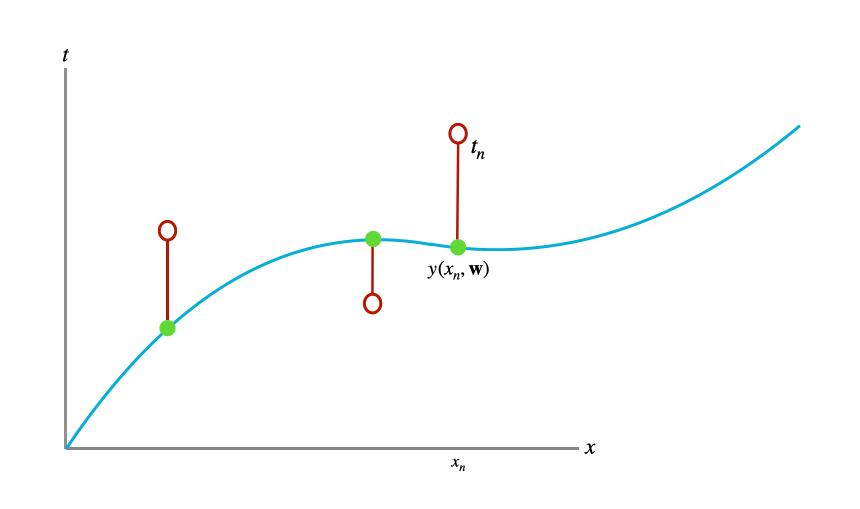
\includegraphics[width=4.16667in,height=\textheight]{./img/sum_of_squares.png}

}

\caption{Figure 1: The sum-of-squares error function in \((3)\) is
computed by taking one half the sum of the squared distances of each
data point from the function \(y(x, \mathbf{w})\). These displacements
are shown in red.}

\end{figure}

Solving for \(\mathbf{w}\) in this setting is fairly straightforward.
Because the error function \((2.2)\) is a quadratic function of the
parameters \(\mathbf{w}\), its derivative with respect to \(\mathbf{w}\)
will be linear in the elements of \(\mathbf{w}\). Therefore, the
minimization of the error function has a unique solution, which we
denote \(\mathbf{w}^*\). It can be found in closed form (Appendix
\textbf{1}). We can then use \(y(x, \mathbf{w}^{*})\) to predict new
values of the target \(t\) for new observed values of the input \(x\).

\hypertarget{overfitting}{%
\subsection{2.3 Overfitting}\label{overfitting}}

There remains the need to choose the order \(M\) of the polynomial,
which falls within the realm of \emph{model selection}. Choosing a large
\(M\) yields a flexible set of models for us to fit, but they are
susceptible to \emph{overfitting}. We will see later that the
least-squares method represents a special case of \emph{maximum
likelihood}, and that overfitting can be viewed as a general symptom of
maximum likelihood.

For now, we can continue with a particular method to avoid overfitting
-- regularization. This involves adding a new term to the error function
\((2.2)\) that penalizes the parameters \(\mathbf{w}\) for being too
large. The simplest penalty term to add is the sum-of-squares of the
\emph{weights}. This leads to a new error function,

\[
\overset{\sim}{E} (\mathbf{w}) = \frac{1}{2} \sum_{n=1}^N \{y(x_n, \mathbf{w}) \}^2 + \frac{\lambda}{2} \lVert \mathbf{w} \rVert^2 \tag{2.3},
\]

where
\(\lVert \mathbf{w} \rVert^2 = \mathbf{w}^\intercal \mathbf{w} = w_0^2 + w_1^2 + \dots + w_M^2\)
and the parameter \(\lambda\) controls the strength of regularization.
Like \((2.2)\), the error function \((2.3)\) can be minimized in close
form (Appendix \textbf{2}). Instituting such a penalty term as we did
takes on different names depending on the literature. In the statistics
literature they are known as shrinkage methods, and in the context of
neural networks it is known as weight decay. Lastly, the specific case
of \((2.3)\) is known as ridge regression.

\hypertarget{a-probabilistic-approach}{%
\section{3 A Probabilistic Approach}\label{a-probabilistic-approach}}

\hypertarget{the-model-1}{%
\subsection{3.1 The Model}\label{the-model-1}}

In the deterministic approach we assumed \(t\) to be the result of a
deterministic function of \(x\) and unknown parameters \(\mathbf{w}\).
We now consider a \emph{probabilistic} model so that we can express
uncertainty in our predictions.

We may not want to make such a strong statement as saying ``\(t\) is
exactly equal to \(y(x, \mathbf{w})\)'' as we did in the previous
section. This could be because we think there is noise in the
observations \(\pmb{\mathsf{t}}\), for example due to measurement error.
To articulate this assumed reality we need to place a distribution over
the target variable \(t\). A sensible distributional assumption is to
place a Gaussian distribution over \(t\) with its mean given by the
parameterized function \(y(x, \mathbf{w})\) and its variance being fixed
and unknown. This is visualized in Figure 2.

\begin{figure}

{\centering 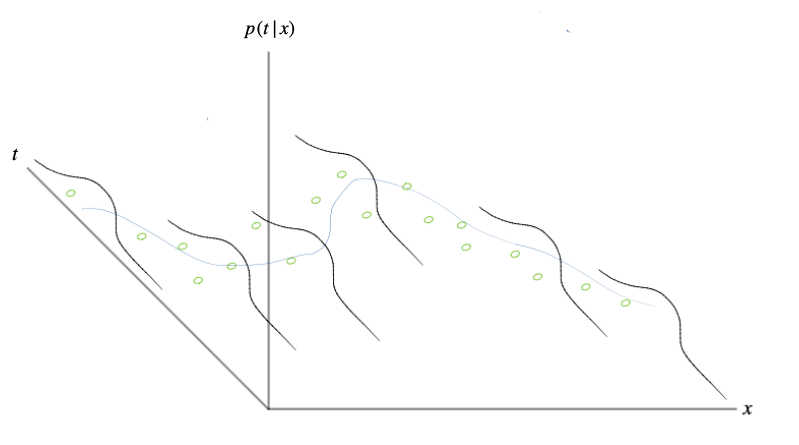
\includegraphics[width=4.16667in,height=\textheight]{./img/gaussian_noise_model.png}

}

\caption{Figure 2: Illustration of a Gaussian conditional distribution
over \(t\) conditioned on \(x\) where the mean of the distribution is
given by some function of \(x\), and the variance is fixed}

\end{figure}

To understand what we're effectively saying when we create such a model,
it is useful to re-emphasize and apply the \emph{data-generating
process} perspective. We can think of our model as describing a process
that produces \(t\) from a given \(x\) and parameter setting
\(\mathbf{w}\). Last section, this process was a deterministic function
\(y(x, \mathbf{w})\). In this section, we extend the process by positing
that each \(t\) is the result of \(y(x, \mathbf{w})\) \emph{and some
additive uncertainty}, where that additive uncertainty takes the form of
a zero-mean Gaussian distribution with unknown variance. This is to say
that we are assuming, to have gotten a particular instance of \(t\):

\begin{itemize}
\tightlist
\item
  we are given an instance of \(x\),
\item
  this instance of \(x\) is then used to obtain the output of the
  parameterized function \(y(x, \mathbf{w})\),
\item
  to which we add a sample from a zero-mean Gaussian with fixed and
  unknown variance.
\end{itemize}

This leads to the following model,

\begin{align}
p(t|x, \mathbf{w}, \beta) &= y(x, \mathbf{w}) + \mathcal{N}(0, \beta^{-1}) \notag \\
&= \mathcal{N}(y(x, \mathbf{w}), \beta^{-1}), \tag{3.1}
\end{align}

where we've used the scaling property of the Gaussian distribution's
mean. \((3.1)\) is an \emph{observation model} and is more specifically
referred to as the \emph{Gaussian noise} model or a \emph{conditional
Gaussian} model.

\hypertarget{maximum-likelihood-estimation}{%
\subsection{3.2 Maximum Likelihood
Estimation}\label{maximum-likelihood-estimation}}

In order to use the training dataset
\(\{\pmb{\mathsf{x}}, \pmb{\mathsf{t}}\}\) to determine the values of
the unknown parameters \(\mathbf{w}\) and \(\beta\), we will use a more
general approach than error minimization -- \emph{maximum likelihood
estimation}. As the name suggests, we will search for a setting of
\(\mathbf{w}\) and \(\beta\) so that the likelihood of our observed data
\(\pmb{\mathsf{t}}\) is maximized. In other words, we've defined a
data-generating process, and we want to find the setting of the
parameters such that the probabilities of our process having
\emph{created} each observed \(t_n \in \pmb{\mathsf{t}}\) from each
\(x_n \in \pmb{\mathsf{x}}\) are maximized. The likelihood measures the
aggregation of all these point-wise probabilities.

In order to use maximum likelihood estimation, we need to have a
\emph{likelihood function}. A likelihood function is \emph{derived} from
an observation model. It can be thought of as an observation model being
\emph{applied} to a particular dataset. Assuming the data
\(\pmb{\mathsf{t}}\) were independently sampled from \((3.1)\), the
likelihood function is the product of evaluating how consistent the
model is with each datapoint \((t_n, x_n)\), and is evaluated for a
particular setting of \(\mathbf{w}\) and \(\beta\),

\[
p(\pmb{\mathsf{t}}| \pmb{\mathsf{x}}, \mathbf{w}, \beta) = \prod_{n=1}^N \mathcal{N}(t_n|y(x_n, \mathbf{w}), \beta^{-1}). \tag{3.2}
\]

Each time we choose a setting for \(\mathbf{w}\) and \(\beta\) and plug
them into our model, we are defining a conditional distribution given by
\((3.1)\). This conditional distribution may agree with the dataset we
have, or it may not. Examples of agreement and disagreement are shown in
Figure 3.

\begin{figure}

{\centering 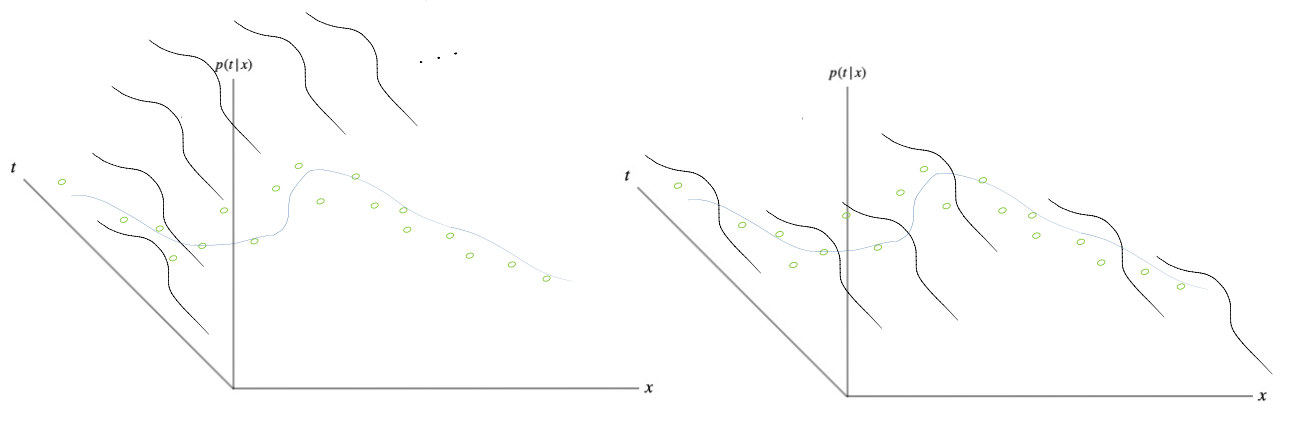
\includegraphics[width=5.20833in,height=\textheight]{./img/gaussian_noise_model_disagreement.png}

}

\caption{Figure 3: A Gaussian noise model shown for a handful of
\(x_i\), with two different settings for \(\mathbf{w}\) and \(\beta\).
On the left is a setting of \((\mathbf{w}, \beta)\) that induces a model
that disagrees with our observed data. On the right is a setting of
\((\mathbf{w}, \beta)\) that induces a model that agrees much better
with our observed data. Maximum likelihood looks for a setting of
\((\mathbf{w}, beta)\) that best agrees with our observed data.}

\end{figure}

We now demonstrate how, in practice, we compute the maximum likelihood
estimates for \(\mathbf{w}\) and \(\beta\). In this example, it can be
done in closed form and amounts to taking the derivative of the
likelihood \((3.2)\), setting it equal to zero, and then solving for
\(\mathbf{w}\) or \(\beta\). We begin with \(\mathbf{w}\). It is common
to instead maximize the log likelihood instead of the likelihood
\((3.2)\) for numerical stability and convenience. We can write the log
likelihood as

\[
\text{ln}p(\pmb{\mathsf{t}}| \pmb{\mathsf{x}}, \mathbf{w}, \beta) = - \frac{\beta}{2} \sum_{n=1}^N \{y(x_n ,\mathbf{w}) - t_n \}^2 + \frac{N}{2} \text{ln}\beta - \frac{N}{2} \text{ln}(2 \pi). \tag{3.3}
\]

\hypertarget{maximum-likelihoods-connection-to-least-squares}{%
\paragraph{\texorpdfstring{\textbf{3.2.1 Maximum Likelihood's connection
to
Least-Squares}}{3.2.1 Maximum Likelihood's connection to Least-Squares}}\label{maximum-likelihoods-connection-to-least-squares}}

In taking the derivative of \((3.3)\) with respect to \(\mathbf{w}\), we
can omit the last two terms as they do not depend on \(\mathbf{w}\). We
can also replace the coefficient \(\frac{\beta}{2}\) with
\(\frac{1}{2}\) since scaling \((3.3)\) by a constant won't change the
location of the maximum of \((3.3)\) with respect to \(\mathbf{w}\).
Lastly, we can equivalently minimize the \emph{negative} log likelihood.
This leaves us with minimizing

\[
\frac{1}{2} \sum_{n=1}^N \{y(x_n, \mathbf{w}) - t_n \}^2. \tag{3.4}
\]

And so we see that the sum-of-squares error function has arisen as a
consequence of maximizing the likelihood under the assumption of a
Gaussian noise distribution. In fact, for a \emph{Gaussian noise model},
maximum likelihood estimation and least-squares estimation find the same
\(\mathbf{w}\); in particular, the one that minimizes \((3.4)\). Once
we've found the maximum likelihood estimate for \(\mathbf{w}\), which we
will denote \(\mathbf{w}_{\text{ML}}\), we can use it to find the
setting for the precision parameter \(\beta\) of the Gaussian
conditional distribution. Maximizing \((3.3)\) with respect to \(\beta\)
yields

\[
\frac{1}{\beta_{\text{ML}}} = \frac{1}{N} \sum_{n=1}^N \{y(x_n, \mathbf{w}_{\text{ML}}) - t_n \}^2. \tag{3.5}
\]

And so we see that the maximum likelihood procedure yields a variance
\(\sigma^2\) as equalling the average squared deviation between the
observed data points and the function \(y(x, \mathbf{w}_{\text{ML}})\).

\hypertarget{maximum-likelihoods-predictive-distribution}{%
\paragraph{\texorpdfstring{\textbf{3.2.2 Maximum Likelihood's predictive
distribution}}{3.2.2 Maximum Likelihood's predictive distribution}}\label{maximum-likelihoods-predictive-distribution}}

The predictive distribution as a result of the maximum likelihood
approach amounts to plugging in the maximum likelihood estimates
\(\mathbf{w}_{\text{ML}}\) and \(\beta_{\text{ML}}\) into the
observation model 3.1:

\[
p(t|x, \mathbf{w}_{\text{ML}}, \beta_{\text{ML}}) = \mathcal{N}(y(x, \mathbf{w}_{\text{ML}}), \beta^{-1}_{\text{ML}}). \tag{3.6}
\]

\hypertarget{maximum-a-posteriori-estimation}{%
\subsection{3.3 Maximum a posteriori
Estimation}\label{maximum-a-posteriori-estimation}}

Introducing a prior distribution over the parameters \(\mathbf{w}\) is a
way of introducing our \emph{prior} beliefs (perhaps through domain
expertise) about the parameters before observing our dataset.
Additionally, as we will see, it serves as a \emph{regularizer} for our
estimate of \(\mathbf{w}\). Importantly, it is also one of the
components in Bayes' theorem, and takes us a step towards a full
Bayesian treatment. For simplicity, we introduce a simple Gaussian prior

\[
p(\mathbf{w}| \alpha) = \mathcal{N}(\mathbf{w} | \mathbf{0}, \alpha^{-1} \mathbf{I}) = \left( \frac{\alpha}{2 \pi} \right)^{(M+1) / 2} \text{exp} \left[- \frac{\alpha}{2} \mathbf{w}^{\intercal} \mathbf{w} \right], \tag{3.7} 
\]

where \(\alpha\) is the precision of the distribution and \(M+1\) is the
number of elements in \(\mathbf{w}\) for an \(M\) order polynomial
function. Variables such as \(\alpha\) are called \emph{hyperparameters}
since we have to choose their values. Now that we have a prior, we can
use Bayes' theorem to yield a quantity proportional to the posterior,

\[
\overbrace{ p(\mathbf{w}|\pmb{\mathsf{x}}, \pmb{\mathsf{t}}, \alpha, \beta) }^{\text{Posterior } p(\mathbf{w}|D)} = \frac{\overbrace{p(\pmb{\mathsf{t}}|\pmb{\mathsf{x}}, \mathbf{w}, \beta)}^{\text{Likelihood } p(D|\mathbf{w})} \; \cdot \; \overbrace{p(\mathbf{w}|\alpha)}^{\text{Prior }p(\mathbf{w})}}{\underbrace{p(\pmb{\mathsf{t}}|\pmb{\mathsf{x}})}_{\text{Model Evidence } p(D)}} \propto \overbrace{p(\pmb{\mathsf{t}}|\pmb{\mathsf{x}}, \mathbf{w}, \beta)}^{\text{Likelihood } p(D|\mathbf{w})} \; \cdot \; \overbrace{p(\mathbf{w}|\alpha)}^{\text{Prior }p(\mathbf{w})}, \tag{3.8}
\]

where the proportion relation \(\propto\) comes from the fact that the
denominator of Bayes' theorem, \(p(D) = p(\mathbf{t} | \mathbf{x})\),
does not depend on \(\mathbf{w}\). Maximizing the right hand size of
\((3.8)\) with respect to \(\mathbf{w}\) is equivalent to maximizing the
posterior with respect to \(\mathbf{w}\) due to the proportionality. By
optimizing \(\mathbf{w}\) to maximize the posterior, we are finding the
most probable parameter values \(\mathbf{w}\) considering our observed
data and also our prior knowledge about \(\mathbf{w}\) encapsulated in
the (data independent) prior \(p(\mathbf{w} | \alpha)\). This yields a
tradeoff between what we believed about \(\mathbf{w}\) before seeing our
data, and the \(\mathbf{w}\) that best fits our data. This technique is
referred to \emph{maximum a posteriori estimation}, MAPE, or MAP.

\hypertarget{maximum-a-posterioris-connection-to-least-squares}{%
\paragraph{\texorpdfstring{\textbf{3.3.1 Maximum a posteriori's
connection to
Least-Squares}}{3.3.1 Maximum a posteriori's connection to Least-Squares}}\label{maximum-a-posterioris-connection-to-least-squares}}

Taking the negative logarithm of \((3.8)\) and combining with the log
likelihood in \((3.3)\) and the prior in \((3.7)\), it can be shown that
the maximum of the posterior is equivalenty the minimum of the following
expression:

\[
\frac{\beta}{2} \sum_{n=1}^N \{y(x_n, \mathbf{w}) - t_n \}^2 + \frac{\alpha}{2} \mathbf{w}^\intercal \mathbf{w}. \tag{3.9}
\]

If we define \(\lambda = \alpha / \beta\), we can rewrite \((3.9)\) as

\[
\frac{1}{2} \sum_{n=1}^N \{y(x_n, \mathbf{w}) - t_n \}^2 + \frac{\lambda}{2} \mathbf{w}^\intercal \mathbf{w}. \tag{3.10}
\]

And so we see that minimizing the regularized sum-of-squares function
introduced in \((4)\) arises naturally from maximizing the posterior of
a Gaussian noise model with Gaussian prior.

Similar to the maximum likelihood section, once we've found the maximum
a posteriori estimate for \(\mathbf{w}\), which we will denote
\(\mathbf{w}_{\text{MAP}}\), we can use it to find the setting for the
precision parameter \(\beta\). We did not introduce a prior over
\(\beta\), so the negative logarithm of the right-hand-side of \((3.8)\)
is

\[
-\text{ln} \left[ \: p(\pmb{\mathsf{t}}|\pmb{\mathsf{x}}, \mathbf{w}, \beta) p(\mathbf{w}|\alpha)  \: \right] = -[ \: \text{ln}p(\pmb{\mathsf{t}}|\pmb{\mathsf{x}}, \mathbf{w}, \beta) + \text{ln} p(\mathbf{w}|\alpha) \: ]. \tag{3.11}
\]

Since we've only gained an additive term that does not functionally
depend on \(\beta\), solving for \(\beta_{\text{MAP}}\) yields a
near-equivalent expression to \((3.5)\) except we now use
\(\mathbf{w}_{\text{MAP}}\) instead of \(\mathbf{w}_{\text{ML}}\):

\[ 
\frac{1}{\beta_{\text{MAP}}} = \frac{1}{N} \sum_{n=1}^{N} \{y(x_n, \mathbf{w}_{\text{MAP}}) - t_n\}^2. \tag{3.12}
\]

\hypertarget{maximum-a-posterioris-predictive-distribution}{%
\paragraph{\texorpdfstring{\textbf{3.3.2 Maximum a posteriori's
predictive
distribution}}{3.3.2 Maximum a posteriori's predictive distribution}}\label{maximum-a-posterioris-predictive-distribution}}

Similar to Maximum Likelihood, the result of the \emph{maximum a
posteriori estimation} method are point-estimates for the parameters
\(\mathbf{w}\) and \(\beta\). We can similarly plug in those estimates,
denoted \(\mathbf{w}_{\text{MAP}}\) and \(\beta_{\text{MAP}}\), into the
observation model \((3.1)\):

\[
p(t|x, \mathbf{w}_{\text{MAP}}, \beta_{\text{MAP}}) = \mathcal{N}(y(x, \mathbf{w}_{\text{MAP}}), \beta^{-1}_{\text{MAP}}). \tag{3.13}
\]

\hypertarget{bayesian-estimation}{%
\subsection{3.4 Bayesian Estimation}\label{bayesian-estimation}}

So far we have been making a point estimate of \(\mathbf{w}\) which does
not yet amount to a Bayesin treatment. In a Bayesian treatment, we take
into account all possible \(\mathbf{w}\) that could have explained our
data. To predict a new value of \(t\) for a new \(x\), we marginalize
over all possible settings of \(\mathbf{w}\), yielding the
\emph{posterior predictive distribution} or \emph{Bayesian model
average}. The goal of the Bayesian treatment is to compute the posterior
over the weights \(p(\mathbf{w}|D)\) which represents all possible
settings of \(\mathbf{w}\) that give rise to models that can explain our
observed data \(D\). To this end, we must use Bayes' theorem:

\[
p(\mathbf{w}|D) = \frac{p(D|\mathbf{w})p(\mathbf{w})}{p(D)}. \tag{3.14}
\]

And for our regression problem in particular, \((3.14)\) can be further
specified as

\[
p(\mathbf{w}|\pmb{\mathsf{t}}, \pmb{\mathsf{x}}, \alpha, \beta) = \frac{\overbrace{p(\pmb{\mathsf{t}} | \pmb{\mathsf{x}}, \mathbf{w}, \beta)}^{\text{Likelihood}} \cdot \overbrace{p(\mathbf{w} | \alpha)}^{\text{Prior}}}{\underbrace{p(\pmb{\mathsf{t}} | \pmb{\mathsf{x}})}_{\text{Evidence}}}.
\tag{3.15} 
\]

To simplify this, we will assume the parameters \(\alpha\) and \(\beta\)
are fixed and known in advance, and we will solely focus on the unknown
\(\mathbf{w}\). \((3.15)\) then turns into

\[
p(\mathbf{w} \vert \pmb{\mathsf{x}}, \pmb{\mathsf{t}}) = \frac{p(\pmb{\mathsf{t}} \vert \pmb{\mathsf{x}}, \mathbf{w}) \cdot p(\mathbf{w})}{p(\pmb{\mathsf{t}} \vert \pmb{\mathsf{x}})}. \tag{3.16}
\]

So instead of computing a single \emph{point estimate} of the weights
(as we've done thus far); now, given the likelihood and the prior, we
can compute the \emph{posterior distribution} over \(\mathbf{w}\) via
Bayes' rule. Computing the posterior can be facilitated by our choice of
prior (a modeling choice) so that we can calculate the posterior in
closed form. Those priors are referred to as \emph{conjugate priors}.
There are a number of other techniques used to instead
\emph{approximate} the posterior
\(p(\mathbf{w}|\pmb{\mathsf{t}}, \pmb{\mathsf{x}})\) when conjugacy is
impossible. These include \emph{variational inference} and \emph{markov
chain monte carlo sampling}. Pretty much all posterior approximation
methods introduce different ways to circumvent the explicit calculation
of the denominator \(P(D) = p(\pmb{\mathsf{t}}|\pmb{\mathsf{x}})\) which
is intractable for any interesting model. We save all these methods for
another post and assume we've found the exact posterior.

\hypertarget{bayesians-predictive-distribution}{%
\paragraph{\texorpdfstring{\textbf{3.4.1 Bayesian's predictive
distribution}}{3.4.1 Bayesian's predictive distribution}}\label{bayesians-predictive-distribution}}

Once it is found, the posterior represents all possible settings of
\(\mathbf{w}\) in that they induce models that can explain our data. To
incorporate this information into a \emph{predictive distribution} so
that we can predict new values of an unobserved \(t\) given an
unobserved \(x\), we marginalize over all possible settings of
\(\mathbf{w}\) like so:

\[
p(t|x, \pmb{\mathsf{x}}, \pmb{\mathsf{t}}) = \int p(t|x, \mathbf{w}) p(\mathbf{w}|\pmb{\mathsf{x}}, \pmb{\mathsf{t}}) \text{d}\mathbf{w}, \tag{3.17}
\]

where \(p(t|x, \mathbf{w})\) is our model given by \((3.1)\) omitting
the dependence on \(\beta\), and
\(p(\mathbf{w}|\pmb{\mathsf{x}}, \pmb{\mathsf{t}})\) is the posterior
over the weights \(\mathbf{w}\). In \((3.15)\),

\begin{itemize}
\tightlist
\item
  we look at a possible setting of \(\mathbf{w}\) which we will denote
  \(\mathbf{w}_i\) according to the posterior
  \(p(\mathbf{w}|\pmb{\mathsf{x}}, \pmb{\mathsf{t}})\). Placing
  \(\mathbf{w}_i\) into our observation model \(p(t|x, \mathbf{w})\)
  defines a ``fitted model'' \(p(t|x, \mathbf{w}_i)\).
\item
  this ``fitted model'' is \emph{multiplied} by the probability of that
  setting of \(\mathbf{w}_i\) given by the posterior. In other words,
  the probability that \(p(t|x, \mathbf{w}_i)\) was used to generate our
  observed data \(\pmb{\mathsf{t}}\) from the inputs
  \(\pmb{\mathsf{x}}\).
\item
  we do this for every possible setting \(\mathbf{w}_i\) according to
  the posterior and integrate.
\end{itemize}

Thus, we are taking a weighted average of all possible ``fitted
models'', where the weights of each component are determined by how
likely the setting of \(\mathbf{w}\) is according to its posterior.

\hypertarget{analyzing-our-specific-predictive-distribution}{%
\paragraph{\texorpdfstring{\textbf{3.4.2 Analyzing our specific
predictive
distribution}}{3.4.2 Analyzing our specific predictive distribution}}\label{analyzing-our-specific-predictive-distribution}}

We will now analyze the specific form of \((3.17)\) for our example
problem. A consequence of us selecting a Gaussian likelihood and a
Gaussian prior is that we can analytically compute the posterior; and it
is Gaussian as well -- an example of \emph{conjugacy}. More so, we can
analytically solve the integration in \((3.17)\) to get a predictive
distribution that itself is Gaussian. In fact, it takes on the more
specific form

\[
p(t|x, \pmb{\mathsf{x}}, \pmb{\mathsf{t}}) = \mathcal{N}(t|m(x), s^2(x)), \tag{3.18}
\]

where the mean and variance are given by

\begin{align}
&m(x) = \beta \pmb{\phi}(x)^{\intercal} \mathbf{S} \sum_{n=1}^N \pmb{\phi}(x_n) t_n \tag{3.19} \\
& s^2(x) = \overbrace{\beta^{-1}}^{\text{noise}} + \underbrace{\pmb{\phi}(x)^\intercal \mathbf{S} \pmb{\phi}(x)}_{\text{Parameter Uncertainty}} \tag{3.20}
\end{align}

\(\mathbf{S}\) is a matrix, and is given by

\[
\mathbf{S}^{-1} = \alpha \mathbf{I} + \beta \sum_{n=1}^N \pmb{\phi}(x_n)  \pmb{\phi}(x),^\intercal \tag{3.21}
\]

where \(\mathbf{I}\) is the unit matrix, and we have defined the vector
\(\pmb{\phi}(x)\) with elements \(\phi_i(x) = x^i\) for \(i=0,...,M\).
In looking at the predictive distribution \((3.16)\), we now see that
the variance depends on \(x\). This is \emph{unlike} the maximum
likelihood predictive distribution \((3.6)\) and the maximum a
posteriori predictive distribution \((3.13)\) where the variance is
fixed for any value of \(x\). It's expansion is described by \((3.20)\)
and it contains two additive components. The first component, as was
already expressed in the maximum likelihood predictive distribution
\(\beta_{\text{ML}}\), is the noise on the target variables. The second
component, which \emph{has not} been expressed until now, arises from
the \emph{uncertainty in the parameters} \(\mathbf{w}\) and is a
consequence of treating \(\mathbf{w}\) as a random variable -- an
artifact of the Bayesian treatment.

\hypertarget{summary}{%
\section{4 Summary}\label{summary}}

\begin{itemize}
\item
  If we assume a Gaussian noise observation model and use maximum
  likelihood to find the setting for the parameters \(\mathbf{w}\), it
  is equivalent to using least-squares to find \(\mathbf{w}\).
\item
  If we assume a Gaussian noise observation model and an Isotropic
  Gaussian prior model on \(\mathbf{w}\), and then use maximum a
  posteriori to find the setting for \(\mathbf{w}\), it is equivalent to
  using least-squares with weight decay regularization to find
  \(\mathbf{w}\).
\item
  If we assume a Gaussian noise observation model and an Isotropic
  Gaussian prior model on \(\mathbf{w}\), and then we use the Bayesian
  approach, we do not find a setting for \(\mathbf{w}\), but rather a
  distribution over \(\mathbf{w}\). This allows us to introduce
  parameter uncertainty in our predictive distribution -- a result of
  many different settings of \(\mathbf{w}\) that could explain the
  training data.
\end{itemize}

\hypertarget{references}{%
\section{References}\label{references}}

\href{https://www.microsoft.com/en-us/research/uploads/prod/2006/01/Bishop-Pattern-Recognition-and-Machine-Learning-2006.pdf}{\emph{Pattern
Recognition and Machine Learning}}, \textbf{Christopher M. Bishop}, 2006

\href{https://www.miketipping.com/papers/met-mlbayes.pdf}{\emph{Bayesian
Inference: An Introduction to Principles and Practice in Machine
Learning}} \textbf{Michael E. Tipping}, 2004

\hypertarget{appendix}{%
\section{Appendix}\label{appendix}}

\hypertarget{solving-for-the-parameters}{%
\subsection{1 Solving for the
parameters}\label{solving-for-the-parameters}}

\hypertarget{analytical-setup}{%
\paragraph{\texorpdfstring{\textbf{1.1 Analytical
Setup}}{1.1 Analytical Setup}}\label{analytical-setup}}

We have the error function
\(E(\mathbf{w}) = \frac{1}{2} \sum_{n=1}^N \{y(x_n, \mathbf{w}) - t_n \}^2\),
where \(y(x, \mathbf{w}) = \sum_{j=0}^M w_j x^j\). We'd like to find the
optimal setting for \(\mathbf{w}\) in the sense that it minimizes
\(E(\mathbf{w})\). We will see that we can cast this minimization
problem as solving a system of linear equations. We will then solve that
system of linear equations with code to attain the optimal
\(\mathbf{w}^{*}\).

\emph{Claim}: The \(w_i\) in \(\mathbf{w} = (w_0, w_1, w_2 ..., w_M)\)
that minimize the error function \(E(\mathbf{w})\) are given by the
solution to the following set of linear equations,

\[
\sum_{j=0}^M A_{ij}w_j = T_i \;\; \text{ where } \;\; A_{ij} = \sum_{n=1}^N(x_n)^{(i+j)}, \; T_i = \sum_{n=1}^N (x_n)^i t_n
\]

\emph{Proof}: We will take the derivative of \(E(\mathbf{w})\) with
respect to \(\mathbf{w}\), set it to zero, and then rearrange terms to
prove the claim above.

By the chain rule,

\[
\frac{\partial E(\mathbf{w})}{\partial w_i} = \frac{\partial E(\mathbf{w})}{\partial y(x_n, \mathbf{w})} \frac{\partial y(x_n, \mathbf{w})}{\partial w_i} \tag{1}
\]

Solving the two terms on the right hand side yields

\[
\begin{aligned}
&\frac{\partial E(\mathbf{w})}{\partial y(x_n, \mathbf{w})} = \sum_{n=1}^N \{y(x_n, \mathbf{w}) - t_n \} \\
&\frac{\partial y(x_n, \mathbf{w})}{\partial w_i} = \frac{\partial}{\partial w_i} (w_0 + w_1x_1 + \dots w_i x_n^i \dots + w_m x_n^M) = x_n^i 
\end{aligned}
\]

Substituting back into \((1)\) yields

\[
\begin{aligned}
\frac{\partial E(\mathbf{w})}{\partial w_i} & = \sum_{n=1}^N \{y(x_n, \mathbf{w}) - t_n \} x_n^i \\ 
& \overset{(i)}{=} \sum_{n=1}^N (\sum_{j=0}^M w_j x_n^{j} - t_n)x_n^i \\
& \overset{(ii)}{=} \sum_{n=1}^N (\sum_{j=0}^M w_j x_n^{i}x_n^j - t_n x_n^i) \\
& \overset{(iii)}{=} \sum_{n=1}^N (\sum_{j=0}^M w_j x_n^{(i+j)} - t_n x_n^i)
\end{aligned}
\]

where in \((\text{i})\) we use the definition of \(y(x_n, \mathbf{w})\),
in \((\text{ii})\) we distribute \(x_n^i\) into the parentheses, and in
\((\text{iii})\) we use the exponent rule. Setting the derivative to
\(0\) and rearranging,

\[
\begin{aligned}
\sum_{n=1}^N (\sum_{j=0}^M w_j x_n^{(i+j)} - t_n x_n^i) & = 0 \\
\sum_{n=1}^N \sum_{j=0}^M w_j x_n^{(i+j)} & = \sum_{n=1}^N t_n x_n^i \\
\sum_{j=0}^M A_{ij}w_j &= T_i
\end{aligned}
\]

\(\blacksquare\)

\hypertarget{code}{%
\paragraph{\texorpdfstring{\textbf{1.2 Code}}{1.2 Code}}\label{code}}

\begin{Shaded}
\begin{Highlighting}[]
\ImportTok{import}\NormalTok{ numpy }\ImportTok{as}\NormalTok{ np}
\ImportTok{import}\NormalTok{ matplotlib.pyplot }\ImportTok{as}\NormalTok{ plt}
\ImportTok{from}\NormalTok{ typing }\ImportTok{import}\NormalTok{ Callable, List, Union, Tuple}

\CommentTok{\# ================ Generating Data ==================== \#}
\KeywordTok{def}\NormalTok{ generate\_data(}
\NormalTok{    seed: }\BuiltInTok{int}\NormalTok{,}
\NormalTok{    signal\_fn: Callable,}
\NormalTok{    noise: }\BuiltInTok{float}\NormalTok{,}
\NormalTok{    num\_samples: }\BuiltInTok{int}\NormalTok{,}
    \BuiltInTok{range}\NormalTok{: List[}\BuiltInTok{float}\NormalTok{],}
\NormalTok{    include\_signal: }\BuiltInTok{bool} \OperatorTok{=} \VariableTok{False}\NormalTok{,}
\NormalTok{    plot: }\BuiltInTok{bool} \OperatorTok{=} \VariableTok{False}\NormalTok{,}
\NormalTok{) }\OperatorTok{{-}\textgreater{}}\NormalTok{ Union[Tuple[Tuple[np.ndarray]], Tuple[np.ndarray]]:}
    \CommentTok{"""}
\CommentTok{    Generate noisy training data and the non{-}noisy data.}

\CommentTok{    Parameters}
\CommentTok{    {-}{-}{-}{-}{-}{-}{-}{-}{-}{-}}
\CommentTok{    seed : int}
\CommentTok{        Seed for reproducibility.}
\CommentTok{    signal\_fn : Callable}
\CommentTok{        A function describing the deterministic data generating process.}
\CommentTok{    noise : float}
\CommentTok{        The \textasciigrave{}scale\textasciigrave{} value for the Gaussian noise to be added.}
\CommentTok{    num\_samples : int}
\CommentTok{        Number of training samples.}
\CommentTok{    range : List[float]}
\CommentTok{        Range of the input variable x.}
\CommentTok{    plot : bool, optional}
\CommentTok{        Whether to plot the data or not, by default False}

\CommentTok{    Returns}
\CommentTok{    {-}{-}{-}{-}{-}{-}{-}}
\CommentTok{    Union[Tuple[Tuple[np.ndarray]], Tuple[np.ndarray]]}
\CommentTok{        If include\_signal = True, two tuples where the first is the noisy}
\CommentTok{        training data and the second is the underlying signal. If include\_signal=False,}
\CommentTok{        then a tuple with just the noisy training data.}
\CommentTok{    """}
    \CommentTok{\# Create generator for reproducible results}
\NormalTok{    generator }\OperatorTok{=}\NormalTok{ np.random.default\_rng(seed)}
    \CommentTok{\# Noisy signal}
\NormalTok{    signal\_noisy\_fn }\OperatorTok{=} \KeywordTok{lambda}\NormalTok{ xs: signal\_fn(xs) }\OperatorTok{+}\NormalTok{ generator.normal(}
\NormalTok{        loc}\OperatorTok{=}\DecValTok{0}\NormalTok{, scale}\OperatorTok{=}\NormalTok{noise, size}\OperatorTok{=}\NormalTok{(num\_samples,)}
\NormalTok{    )}
    \CommentTok{\# Create training data}
\NormalTok{    xs }\OperatorTok{=}\NormalTok{ np.linspace(start}\OperatorTok{=}\BuiltInTok{range}\NormalTok{[}\DecValTok{0}\NormalTok{], stop}\OperatorTok{=}\BuiltInTok{range}\NormalTok{[}\DecValTok{1}\NormalTok{], num}\OperatorTok{=}\NormalTok{num\_samples)}
\NormalTok{    ts }\OperatorTok{=}\NormalTok{ signal\_noisy\_fn(xs)}
    \ControlFlowTok{if}\NormalTok{ include\_signal:}
        \CommentTok{\# Create "signal"}
\NormalTok{        x\_axis }\OperatorTok{=}\NormalTok{ np.linspace(start}\OperatorTok{=}\DecValTok{0}\NormalTok{, stop}\OperatorTok{=}\DecValTok{1}\NormalTok{, num}\OperatorTok{=}\DecValTok{1000}\NormalTok{)}
\NormalTok{        signal }\OperatorTok{=}\NormalTok{ signal\_fn(x\_axis)}
\NormalTok{        to\_return }\OperatorTok{=}\NormalTok{ ((xs, ts), (x\_axis, signal))}
    \ControlFlowTok{else}\NormalTok{:}
\NormalTok{        to\_return }\OperatorTok{=}\NormalTok{ (xs, ts)}
    \ControlFlowTok{if}\NormalTok{ plot:}
        \CommentTok{\# ===== Plot Data ====== \#}
        \CommentTok{\# Create figure}
\NormalTok{        figure1 }\OperatorTok{=}\NormalTok{ plt.figure(figsize}\OperatorTok{=}\NormalTok{(}\DecValTok{8}\NormalTok{, }\DecValTok{4}\NormalTok{))}
\NormalTok{        plt.axis(}\StringTok{"off"}\NormalTok{)}
        \CommentTok{\# Plot Signal}
\NormalTok{        line }\OperatorTok{=}\NormalTok{ np.linspace(start}\OperatorTok{=}\DecValTok{0}\NormalTok{, stop}\OperatorTok{=}\DecValTok{1}\NormalTok{, num}\OperatorTok{=}\DecValTok{1000}\NormalTok{)}
\NormalTok{        plt.plot(x\_axis, signal, c}\OperatorTok{=}\StringTok{"green"}\NormalTok{)}
        \CommentTok{\# Plot training data}
\NormalTok{        plt.scatter(xs, ts, c}\OperatorTok{=}\StringTok{"black"}\NormalTok{)}
\NormalTok{        plt.show()}
    \ControlFlowTok{return}\NormalTok{ to\_return}

\CommentTok{\# ============= Solving for w ====================== \#}
\KeywordTok{def}\NormalTok{ create\_A(xs: np.array, M: }\BuiltInTok{int}\NormalTok{) }\OperatorTok{{-}\textgreater{}}\NormalTok{ np.array:}
    \CommentTok{"""}
\CommentTok{    Create the matrix A where A\_ij = sum\_n=1\^{}N [x\_n\^{}(i+j)].}
\CommentTok{    """}
\NormalTok{    A }\OperatorTok{=}\NormalTok{ np.zeros((M, M))}
    \ControlFlowTok{for}\NormalTok{ i }\KeywordTok{in} \BuiltInTok{range}\NormalTok{(M):}
        \ControlFlowTok{for}\NormalTok{ j }\KeywordTok{in} \BuiltInTok{range}\NormalTok{(M):}
\NormalTok{            A[i][j] }\OperatorTok{=}\NormalTok{ np.}\BuiltInTok{sum}\NormalTok{(xs }\OperatorTok{**}\NormalTok{ (i }\OperatorTok{+}\NormalTok{ j))}
    \ControlFlowTok{return}\NormalTok{ A}


\KeywordTok{def}\NormalTok{ create\_T(xs: np.array, ts: np.array, M: }\BuiltInTok{int}\NormalTok{) }\OperatorTok{{-}\textgreater{}}\NormalTok{ np.array:}
    \CommentTok{"""}
\CommentTok{    Create the vector T where T\_i = sum\_n=1\^{}N (x\_n\^{}i) t\_n.}
\CommentTok{    """}
\NormalTok{    T }\OperatorTok{=}\NormalTok{ np.zeros((M,))}
    \ControlFlowTok{for}\NormalTok{ i }\KeywordTok{in} \BuiltInTok{range}\NormalTok{(M):}
\NormalTok{        T[i] }\OperatorTok{=}\NormalTok{ np.}\BuiltInTok{sum}\NormalTok{((xs}\OperatorTok{**}\NormalTok{i) }\OperatorTok{*}\NormalTok{ ts)}
    \ControlFlowTok{return}\NormalTok{ T}


\KeywordTok{def}\NormalTok{ create\_lambdaI(size: }\BuiltInTok{int}\NormalTok{, ln\_lambda: }\BuiltInTok{float}\NormalTok{) }\OperatorTok{{-}\textgreater{}}\NormalTok{ np.array:}
    \CommentTok{"""}
\CommentTok{    Create an identity matrix with lambda as the diagonal elements.}
\CommentTok{    """}
\NormalTok{    lambda\_ }\OperatorTok{=}\NormalTok{ np.exp(ln\_lambda)}
\NormalTok{    identity }\OperatorTok{=}\NormalTok{ np.eye(N}\OperatorTok{=}\NormalTok{size)}
    \ControlFlowTok{return}\NormalTok{ lambda\_ }\OperatorTok{*}\NormalTok{ identity}


\KeywordTok{def}\NormalTok{ solve\_for\_w(}
\NormalTok{    xs: np.array, ts: np.array, M: }\BuiltInTok{int}\NormalTok{, ln\_lambda: }\BuiltInTok{float} \OperatorTok{=} \VariableTok{None}
\NormalTok{) }\OperatorTok{{-}\textgreater{}}\NormalTok{ np.array:}
    \CommentTok{"""}
\CommentTok{    Creates A and T using \textasciigrave{}create\_A\textasciigrave{} and \textasciigrave{}create\_T\textasciigrave{} and then solves}
\CommentTok{    the linear system of equations to get w.}
\CommentTok{    """}
\NormalTok{    A }\OperatorTok{=}\NormalTok{ create\_A(xs}\OperatorTok{=}\NormalTok{xs, M}\OperatorTok{=}\NormalTok{M)}
\NormalTok{    T }\OperatorTok{=}\NormalTok{ create\_T(xs}\OperatorTok{=}\NormalTok{xs, ts}\OperatorTok{=}\NormalTok{ts, M}\OperatorTok{=}\NormalTok{M)}
    \ControlFlowTok{if}\NormalTok{ ln\_lambda:}
\NormalTok{        lambdaI }\OperatorTok{=}\NormalTok{ create\_lambdaI(size}\OperatorTok{=}\NormalTok{M, ln\_lambda}\OperatorTok{=}\NormalTok{ln\_lambda)}
\NormalTok{        A\_plus\_lambdaI }\OperatorTok{=}\NormalTok{ A }\OperatorTok{+}\NormalTok{ lambdaI}
        \ControlFlowTok{return}\NormalTok{ np.linalg.solve(a}\OperatorTok{=}\NormalTok{A\_plus\_lambdaI, b}\OperatorTok{=}\NormalTok{T)}
    \ControlFlowTok{else}\NormalTok{:}
        \ControlFlowTok{return}\NormalTok{ np.linalg.solve(a}\OperatorTok{=}\NormalTok{A, b}\OperatorTok{=}\NormalTok{T)}

\CommentTok{\# ============== Prediction ====================== \#}
\KeywordTok{def}\NormalTok{ predict(w: np.array, x: np.array, M) }\OperatorTok{{-}\textgreater{}}\NormalTok{ np.array:}
    \CommentTok{"""}
\CommentTok{    Feature expand the input x and then run the linear}
\CommentTok{    transformation involving w,x to get predictions for target t.}
\CommentTok{    """}
    \CommentTok{\# Get [x**1, x**2, x**3 ... x**M] for each x}
\NormalTok{    N }\OperatorTok{=}\NormalTok{ x.shape[}\DecValTok{0}\NormalTok{]}
\NormalTok{    powers }\OperatorTok{=}\NormalTok{ np.arange(}\DecValTok{0}\NormalTok{, M)}
\NormalTok{    powers\_expanded }\OperatorTok{=}\NormalTok{ np.tile(powers, (N,)).reshape(N, M)}
\NormalTok{    xs\_expanded }\OperatorTok{=}\NormalTok{ x.repeat(M).reshape(N, M)}
\NormalTok{    xs\_powered }\OperatorTok{=}\NormalTok{ np.power(xs\_expanded, powers\_expanded)}
    \CommentTok{\# Apply w}
    \ControlFlowTok{return}\NormalTok{ w }\OperatorTok{@}\NormalTok{ xs\_powered.T}

\CommentTok{\# ========== Main =========== \#}
\NormalTok{(xs, ts), (x\_axis, signal\_values) }\OperatorTok{=}\NormalTok{ generate\_data(}
\NormalTok{    seed}\OperatorTok{=}\DecValTok{123}\NormalTok{,}
\NormalTok{    signal\_fn}\OperatorTok{=}\KeywordTok{lambda}\NormalTok{ x: np.sin(}\DecValTok{2} \OperatorTok{*}\NormalTok{ np.pi }\OperatorTok{*}\NormalTok{ x),}
\NormalTok{    noise}\OperatorTok{=}\FloatTok{0.5}\NormalTok{,}
\NormalTok{    num\_samples}\OperatorTok{=}\DecValTok{20}\NormalTok{,}
    \BuiltInTok{range}\OperatorTok{=}\NormalTok{[}\DecValTok{0}\NormalTok{, }\DecValTok{1}\NormalTok{],}
\NormalTok{    include\_signal}\OperatorTok{=}\VariableTok{True}\NormalTok{,}
\NormalTok{    plot}\OperatorTok{=}\VariableTok{False}\NormalTok{,}
\NormalTok{)}

\NormalTok{figure }\OperatorTok{=}\NormalTok{ plt.figure(figsize}\OperatorTok{=}\NormalTok{(}\DecValTok{8}\NormalTok{, }\DecValTok{8}\NormalTok{))}
\NormalTok{cols, rows }\OperatorTok{=} \DecValTok{2}\NormalTok{, }\DecValTok{4}
\ControlFlowTok{for}\NormalTok{ i }\KeywordTok{in} \BuiltInTok{range}\NormalTok{(}\DecValTok{1}\NormalTok{, cols }\OperatorTok{*}\NormalTok{ rows }\OperatorTok{+} \DecValTok{1}\NormalTok{):}
\NormalTok{    M }\OperatorTok{=}\NormalTok{ i }\OperatorTok{+} \DecValTok{1}
\NormalTok{    w }\OperatorTok{=}\NormalTok{ solve\_for\_w(xs}\OperatorTok{=}\NormalTok{xs, ts}\OperatorTok{=}\NormalTok{ts, M}\OperatorTok{=}\NormalTok{M)}
\NormalTok{    t\_hats }\OperatorTok{=}\NormalTok{ predict(w, x\_axis, M)}
\NormalTok{    figure.add\_subplot(rows, cols, i)}
\NormalTok{    plt.axis(}\StringTok{"off"}\NormalTok{)}
\NormalTok{    plt.title(}\SpecialStringTok{f"M = }\SpecialCharTok{\{}\NormalTok{M}\SpecialCharTok{\}}\SpecialStringTok{"}\NormalTok{)}
    \CommentTok{\# Plot signal}
\NormalTok{    plt.plot(x\_axis, signal\_values, label}\OperatorTok{=}\StringTok{"Signal"}\NormalTok{, c}\OperatorTok{=}\StringTok{"green"}\NormalTok{)}
    \CommentTok{\# Plot data}
\NormalTok{    plt.scatter(xs, ts, s}\OperatorTok{=}\DecValTok{3}\NormalTok{, label}\OperatorTok{=}\StringTok{"Data"}\NormalTok{, c}\OperatorTok{=}\StringTok{"black"}\NormalTok{)}
    \CommentTok{\# Plot predictions}
\NormalTok{    plt.plot(x\_axis, t\_hats, label}\OperatorTok{=}\StringTok{"Predicted Signal"}\NormalTok{)}
\NormalTok{plt.show()}
\end{Highlighting}
\end{Shaded}

\begin{figure}

{\centering 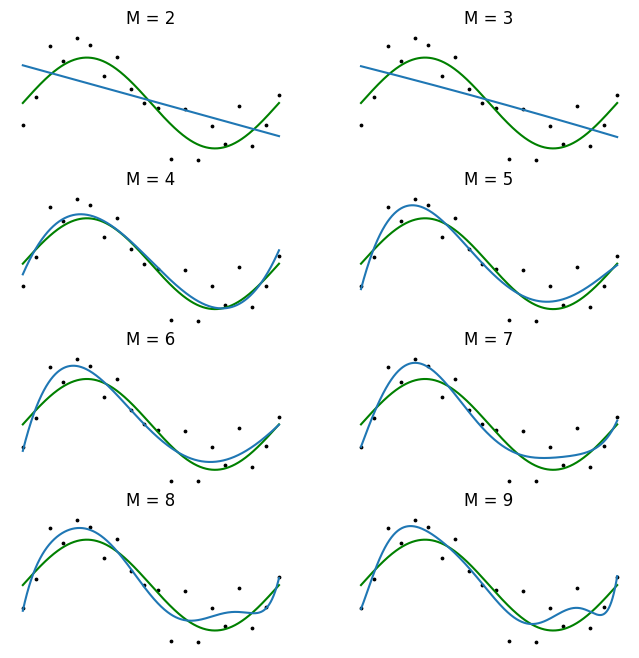
\includegraphics[width=5.20833in,height=\textheight]{./img/mle_w.png}

}

\caption{Signal (green), training data (black), and fitted curves (blue)
for various settings of M -- the order of the polynomial.}

\end{figure}

\hypertarget{solving-for-the-parameters-with-a-penalty-term}{%
\subsection{2 Solving for the parameters with a penalty
term}\label{solving-for-the-parameters-with-a-penalty-term}}

\hypertarget{analytical-setup-1}{%
\paragraph{\texorpdfstring{\textbf{2.1 Analytical
Setup}}{2.1 Analytical Setup}}\label{analytical-setup-1}}

We have the error function
\(\overset{\sim}{E} (\mathbf{w}) = \frac{1}{2} \sum_{n=1}^N \{y(x_n, \mathbf{w}) \}^2 + \frac{\lambda}{2} \lVert \mathbf{w} \rVert^2\),
where
\(\lVert \mathbf{w} \rVert^2 = \mathbf{w}^\intercal \mathbf{w} = w_0^2 + w_1^2 + \dots + w_M^2\)
and the parameter \(\lambda\) controls the strength of regularization.
We'd like to find the optimal setting for \(\mathbf{w}\) in the sense
that it minimizes \(\overset{\sim}{E} (\mathbf{w})\). We will see that
we can cast this minimization problem as solving a system of linear
equations. We will then solve that system of linear equations with code
to attain the optimal \(\mathbf{w}^{*}\).

\emph{Claim}: The \(w_i\) in \(\mathbf{w} = (w_1, w_2, ..., w_M)\) that
minimize the error function \(\overset{\sim}{E} (\mathbf{w})\) are given
by the solution to the following set of linear equations,

\[
\sum_{j=0}^M A_{ij}w_j + \lambda w_i = T_i \;\; \text{ where } \;\; A_{ij} = \sum_{n=1}^N(x_n)^{(i+j)}, \; T_i = \sum_{n=1}^N (x_n)^i t_n
\]

\emph{Proof}: We will take the derivative of
\(\overset{\sim}{E} (\mathbf{w})\) with respect to \(\mathbf{w}\), set
it to zero, and then rearrange terms to prove the claim above.

By the chain rule,

\[
\frac{\partial \overset{\sim}{E}(\mathbf{w})}{\partial w_i} = \frac{\partial E(\mathbf{w})}{\partial y(x_n, \mathbf{w})} \frac{\partial y(x_n, \mathbf{w})}{\partial w_i} + \frac{\lambda}{2} \frac{\partial \mathbf{w}^\intercal \mathbf{w}}{\partial w_i} \tag{2}
\]

Solving the two terms on the right hand side yields

\[
\begin{aligned}
&\frac{\partial \overset{\sim}{E}(\mathbf{w})}{\partial y(x_n, \mathbf{w})} = \sum_{n=1}^N \{y(x_n, \mathbf{w}) - t_n \} \\
&\frac{\partial y(x_n, \mathbf{w})}{\partial w_i} = \frac{\partial}{\partial w_i} (w_0 + w_1x_1 + \dots w_i x_n^i \dots + w_m x_n^M) = x_n^i \\
&\frac{\partial \mathbf{w}^\intercal \mathbf{w}}{\partial w_i} = \frac{\partial}{\partial w_i} (w_0^2 + w_1^2 + \dots w_i^2 + \dots w_M^2) = 2 w_i
\end{aligned}
\]

Substituting back into \((2)\) yields

\[
\begin{aligned}
\frac{\partial \overset{\sim}{E}(\mathbf{w})}{\partial w_i} & = \sum_{n=1}^N \{y(x_n, \mathbf{w}) - t_n \} x_n^i + \frac{\lambda}{2} 2 w_i \\
& \overset{(i)}{=} \sum_{n=1}^N (\sum_{j=0}^M w_j x_n^{j} - t_n)x_n^i + \lambda w_i  \\
& \overset{(ii)}{=} \sum_{n=1}^N (\sum_{j=0}^M w_j x_n^{i}x_n^j - t_n x_n^i) + \lambda w_i  \\
& \overset{(iii)}{=} \sum_{n=1}^N (\sum_{j=0}^M w_j x_n^{(i+j)} - t_n x_n^i) + \lambda w_i 
\end{aligned}
\]

where in \((\text{i})\) we use the definition of \(y(x_n, \mathbf{w})\)
and \(\frac{\lambda}{2} \cdot 2 = \lambda\), in \((\text{ii})\) we
distribute \(x_n^i\) into the parentheses, and in \((\text{iii})\) we
use the exponent rule. Setting the derivative to \(0\) and rearranging,

\[
\begin{aligned}
\sum_{n=1}^N (\sum_{j=0}^M w_j x_n^{(i+j)} - t_n x_n^i) + \lambda w_i & = 0 \\
\sum_{n=1}^N \sum_{j=0}^M w_j x_n^{(i+j)} + \lambda w_i & = \sum_{n=1}^N t_n x_n^i \\
\sum_{j=0}^M A_{ij}w_j + \lambda w_i &= T_i
\end{aligned}
\]

\(\blacksquare\)

\hypertarget{code-1}{%
\paragraph{\texorpdfstring{\textbf{2.2 Code}}{2.2 Code}}\label{code-1}}

\begin{Shaded}
\begin{Highlighting}[]
\ImportTok{import}\NormalTok{ numpy }\ImportTok{as}\NormalTok{ np}
\ImportTok{import}\NormalTok{ matplotlib.pyplot }\ImportTok{as}\NormalTok{ plt}
\ImportTok{from}\NormalTok{ typing }\ImportTok{import}\NormalTok{ Callable, List, Union, Tuple}

\CommentTok{\# ================ Generating Data ==================== \#}
\KeywordTok{def}\NormalTok{ generate\_data(}
\NormalTok{    seed: }\BuiltInTok{int}\NormalTok{,}
\NormalTok{    signal\_fn: Callable,}
\NormalTok{    noise: }\BuiltInTok{float}\NormalTok{,}
\NormalTok{    num\_samples: }\BuiltInTok{int}\NormalTok{,}
    \BuiltInTok{range}\NormalTok{: List[}\BuiltInTok{float}\NormalTok{],}
\NormalTok{    include\_signal: }\BuiltInTok{bool} \OperatorTok{=} \VariableTok{False}\NormalTok{,}
\NormalTok{    plot: }\BuiltInTok{bool} \OperatorTok{=} \VariableTok{False}\NormalTok{,}
\NormalTok{) }\OperatorTok{{-}\textgreater{}}\NormalTok{ Union[Tuple[Tuple[np.ndarray]], Tuple[np.ndarray]]:}
    \CommentTok{"""}
\CommentTok{    Generate noisy training data and the non{-}noisy data.}

\CommentTok{    Parameters}
\CommentTok{    {-}{-}{-}{-}{-}{-}{-}{-}{-}{-}}
\CommentTok{    seed : int}
\CommentTok{        Seed for reproducibility.}
\CommentTok{    signal\_fn : Callable}
\CommentTok{        A function describing the deterministic data generating process.}
\CommentTok{    noise : float}
\CommentTok{        The \textasciigrave{}scale\textasciigrave{} value for the Gaussian noise to be added.}
\CommentTok{    num\_samples : int}
\CommentTok{        Number of training samples.}
\CommentTok{    range : List[float]}
\CommentTok{        Range of the input variable x.}
\CommentTok{    plot : bool, optional}
\CommentTok{        Whether to plot the data or not, by default False}

\CommentTok{    Returns}
\CommentTok{    {-}{-}{-}{-}{-}{-}{-}}
\CommentTok{    Union[Tuple[Tuple[np.ndarray]], Tuple[np.ndarray]]}
\CommentTok{        If include\_signal = True, two tuples where the first is the noisy}
\CommentTok{        training data and the second is the underlying signal. If include\_signal=False,}
\CommentTok{        then a tuple with just the noisy training data.}
\CommentTok{    """}
    \CommentTok{\# Create generator for reproducible results}
\NormalTok{    generator }\OperatorTok{=}\NormalTok{ np.random.default\_rng(seed)}
    \CommentTok{\# Noisy signal}
\NormalTok{    signal\_noisy\_fn }\OperatorTok{=} \KeywordTok{lambda}\NormalTok{ xs: signal\_fn(xs) }\OperatorTok{+}\NormalTok{ generator.normal(}
\NormalTok{        loc}\OperatorTok{=}\DecValTok{0}\NormalTok{, scale}\OperatorTok{=}\NormalTok{noise, size}\OperatorTok{=}\NormalTok{(num\_samples,)}
\NormalTok{    )}
    \CommentTok{\# Create training data}
\NormalTok{    xs }\OperatorTok{=}\NormalTok{ np.linspace(start}\OperatorTok{=}\BuiltInTok{range}\NormalTok{[}\DecValTok{0}\NormalTok{], stop}\OperatorTok{=}\BuiltInTok{range}\NormalTok{[}\DecValTok{1}\NormalTok{], num}\OperatorTok{=}\NormalTok{num\_samples)}
\NormalTok{    ts }\OperatorTok{=}\NormalTok{ signal\_noisy\_fn(xs)}
    \ControlFlowTok{if}\NormalTok{ include\_signal:}
        \CommentTok{\# Create "signal"}
\NormalTok{        x\_axis }\OperatorTok{=}\NormalTok{ np.linspace(start}\OperatorTok{=}\DecValTok{0}\NormalTok{, stop}\OperatorTok{=}\DecValTok{1}\NormalTok{, num}\OperatorTok{=}\DecValTok{1000}\NormalTok{)}
\NormalTok{        signal }\OperatorTok{=}\NormalTok{ signal\_fn(x\_axis)}
\NormalTok{        to\_return }\OperatorTok{=}\NormalTok{ ((xs, ts), (x\_axis, signal))}
    \ControlFlowTok{else}\NormalTok{:}
\NormalTok{        to\_return }\OperatorTok{=}\NormalTok{ (xs, ts)}
    \ControlFlowTok{if}\NormalTok{ plot:}
        \CommentTok{\# ===== Plot Data ====== \#}
        \CommentTok{\# Create figure}
\NormalTok{        figure1 }\OperatorTok{=}\NormalTok{ plt.figure(figsize}\OperatorTok{=}\NormalTok{(}\DecValTok{8}\NormalTok{, }\DecValTok{4}\NormalTok{))}
\NormalTok{        plt.axis(}\StringTok{"off"}\NormalTok{)}
        \CommentTok{\# Plot Signal}
\NormalTok{        line }\OperatorTok{=}\NormalTok{ np.linspace(start}\OperatorTok{=}\DecValTok{0}\NormalTok{, stop}\OperatorTok{=}\DecValTok{1}\NormalTok{, num}\OperatorTok{=}\DecValTok{1000}\NormalTok{)}
\NormalTok{        plt.plot(x\_axis, signal, c}\OperatorTok{=}\StringTok{"green"}\NormalTok{)}
        \CommentTok{\# Plot training data}
\NormalTok{        plt.scatter(xs, ts, c}\OperatorTok{=}\StringTok{"black"}\NormalTok{)}
\NormalTok{        plt.show()}
    \ControlFlowTok{return}\NormalTok{ to\_return}

\CommentTok{\# ============= Solving for w ====================== \#}
\KeywordTok{def}\NormalTok{ create\_A(xs: np.array, M: }\BuiltInTok{int}\NormalTok{) }\OperatorTok{{-}\textgreater{}}\NormalTok{ np.array:}
    \CommentTok{"""}
\CommentTok{    Create the matrix A where A\_ij = sum\_n=1\^{}N [x\_n\^{}(i+j)].}
\CommentTok{    """}
\NormalTok{    A }\OperatorTok{=}\NormalTok{ np.zeros((M, M))}
    \ControlFlowTok{for}\NormalTok{ i }\KeywordTok{in} \BuiltInTok{range}\NormalTok{(M):}
        \ControlFlowTok{for}\NormalTok{ j }\KeywordTok{in} \BuiltInTok{range}\NormalTok{(M):}
\NormalTok{            A[i][j] }\OperatorTok{=}\NormalTok{ np.}\BuiltInTok{sum}\NormalTok{(xs }\OperatorTok{**}\NormalTok{ (i }\OperatorTok{+}\NormalTok{ j))}
    \ControlFlowTok{return}\NormalTok{ A}


\KeywordTok{def}\NormalTok{ create\_T(xs: np.array, ts: np.array, M: }\BuiltInTok{int}\NormalTok{) }\OperatorTok{{-}\textgreater{}}\NormalTok{ np.array:}
    \CommentTok{"""}
\CommentTok{    Create the vector T where T\_i = sum\_n=1\^{}N (x\_n\^{}i) t\_n.}
\CommentTok{    """}
\NormalTok{    T }\OperatorTok{=}\NormalTok{ np.zeros((M,))}
    \ControlFlowTok{for}\NormalTok{ i }\KeywordTok{in} \BuiltInTok{range}\NormalTok{(M):}
\NormalTok{        T[i] }\OperatorTok{=}\NormalTok{ np.}\BuiltInTok{sum}\NormalTok{((xs}\OperatorTok{**}\NormalTok{i) }\OperatorTok{*}\NormalTok{ ts)}
    \ControlFlowTok{return}\NormalTok{ T}


\KeywordTok{def}\NormalTok{ create\_lambdaI(size: }\BuiltInTok{int}\NormalTok{, ln\_lambda: }\BuiltInTok{float}\NormalTok{) }\OperatorTok{{-}\textgreater{}}\NormalTok{ np.array:}
    \CommentTok{"""}
\CommentTok{    Create an identity matrix with lambda as the diagonal elements.}
\CommentTok{    """}
\NormalTok{    lambda\_ }\OperatorTok{=}\NormalTok{ np.exp(ln\_lambda)}
\NormalTok{    identity }\OperatorTok{=}\NormalTok{ np.eye(N}\OperatorTok{=}\NormalTok{size)}
    \ControlFlowTok{return}\NormalTok{ lambda\_ }\OperatorTok{*}\NormalTok{ identity}


\KeywordTok{def}\NormalTok{ solve\_for\_w(}
\NormalTok{    xs: np.array, ts: np.array, M: }\BuiltInTok{int}\NormalTok{, ln\_lambda: }\BuiltInTok{float} \OperatorTok{=} \VariableTok{None}
\NormalTok{) }\OperatorTok{{-}\textgreater{}}\NormalTok{ np.array:}
    \CommentTok{"""}
\CommentTok{    Creates A and T using \textasciigrave{}create\_A\textasciigrave{} and \textasciigrave{}create\_T\textasciigrave{} and then solves}
\CommentTok{    the linear system of equations to get w.}
\CommentTok{    """}
\NormalTok{    A }\OperatorTok{=}\NormalTok{ create\_A(xs}\OperatorTok{=}\NormalTok{xs, M}\OperatorTok{=}\NormalTok{M)}
\NormalTok{    T }\OperatorTok{=}\NormalTok{ create\_T(xs}\OperatorTok{=}\NormalTok{xs, ts}\OperatorTok{=}\NormalTok{ts, M}\OperatorTok{=}\NormalTok{M)}
    \ControlFlowTok{if}\NormalTok{ ln\_lambda:}
\NormalTok{        lambdaI }\OperatorTok{=}\NormalTok{ create\_lambdaI(size}\OperatorTok{=}\NormalTok{M, ln\_lambda}\OperatorTok{=}\NormalTok{ln\_lambda)}
\NormalTok{        A\_plus\_lambdaI }\OperatorTok{=}\NormalTok{ A }\OperatorTok{+}\NormalTok{ lambdaI}
        \ControlFlowTok{return}\NormalTok{ np.linalg.solve(a}\OperatorTok{=}\NormalTok{A\_plus\_lambdaI, b}\OperatorTok{=}\NormalTok{T)}
    \ControlFlowTok{else}\NormalTok{:}
        \ControlFlowTok{return}\NormalTok{ np.linalg.solve(a}\OperatorTok{=}\NormalTok{A, b}\OperatorTok{=}\NormalTok{T)}

\CommentTok{\# ============== Prediction ====================== \#}
\KeywordTok{def}\NormalTok{ predict(w: np.array, x: np.array, M) }\OperatorTok{{-}\textgreater{}}\NormalTok{ np.array:}
    \CommentTok{"""}
\CommentTok{    Feature expand the input x and then run the linear}
\CommentTok{    transformation involving w,x to get predictions for target t.}
\CommentTok{    """}
    \CommentTok{\# Get [x**1, x**2, x**3 ... x**M] for each x}
\NormalTok{    N }\OperatorTok{=}\NormalTok{ x.shape[}\DecValTok{0}\NormalTok{]}
\NormalTok{    powers }\OperatorTok{=}\NormalTok{ np.arange(}\DecValTok{0}\NormalTok{, M)}
\NormalTok{    powers\_expanded }\OperatorTok{=}\NormalTok{ np.tile(powers, (N,)).reshape(N, M)}
\NormalTok{    xs\_expanded }\OperatorTok{=}\NormalTok{ x.repeat(M).reshape(N, M)}
\NormalTok{    xs\_powered }\OperatorTok{=}\NormalTok{ np.power(xs\_expanded, powers\_expanded)}
    \CommentTok{\# Apply w}
    \ControlFlowTok{return}\NormalTok{ w }\OperatorTok{@}\NormalTok{ xs\_powered.T}

\CommentTok{\# ============= Main ================== \#}
\NormalTok{(xs, ts), (x\_axis, signal\_values) }\OperatorTok{=}\NormalTok{ generate\_data(}
\NormalTok{    seed}\OperatorTok{=}\DecValTok{123}\NormalTok{,}
\NormalTok{    signal\_fn}\OperatorTok{=}\KeywordTok{lambda}\NormalTok{ x: np.sin(}\DecValTok{2} \OperatorTok{*}\NormalTok{ np.pi }\OperatorTok{*}\NormalTok{ x),}
\NormalTok{    noise}\OperatorTok{=}\FloatTok{0.5}\NormalTok{,}
\NormalTok{    num\_samples}\OperatorTok{=}\DecValTok{20}\NormalTok{,}
    \BuiltInTok{range}\OperatorTok{=}\NormalTok{[}\DecValTok{0}\NormalTok{, }\DecValTok{1}\NormalTok{],}
\NormalTok{    include\_signal}\OperatorTok{=}\VariableTok{False}\NormalTok{,}
\NormalTok{    plot}\OperatorTok{=}\VariableTok{True}\NormalTok{,}
\NormalTok{)}

\NormalTok{figure }\OperatorTok{=}\NormalTok{ plt.figure(figsize}\OperatorTok{=}\NormalTok{(}\DecValTok{8}\NormalTok{, }\DecValTok{8}\NormalTok{))}
\NormalTok{cols, rows }\OperatorTok{=} \DecValTok{2}\NormalTok{, }\DecValTok{4}
\ControlFlowTok{for}\NormalTok{ i }\KeywordTok{in} \BuiltInTok{range}\NormalTok{(}\DecValTok{1}\NormalTok{, cols }\OperatorTok{*}\NormalTok{ rows }\OperatorTok{+} \DecValTok{1}\NormalTok{):}
\NormalTok{    M }\OperatorTok{=}\NormalTok{ i }\OperatorTok{+} \DecValTok{1}
\NormalTok{    w }\OperatorTok{=}\NormalTok{ solve\_for\_w(xs}\OperatorTok{=}\NormalTok{xs, ts}\OperatorTok{=}\NormalTok{ts, M}\OperatorTok{=}\NormalTok{M, ln\_lambda}\OperatorTok{={-}}\DecValTok{8}\NormalTok{)}
\NormalTok{    t\_hats }\OperatorTok{=}\NormalTok{ predict(w, x\_axis, M)}
\NormalTok{    figure.add\_subplot(rows, cols, i)}
\NormalTok{    plt.axis(}\StringTok{"off"}\NormalTok{)}
\NormalTok{    plt.title(}\SpecialStringTok{f"M = }\SpecialCharTok{\{}\NormalTok{M}\SpecialCharTok{\}}\SpecialStringTok{"}\NormalTok{)}
    \CommentTok{\# Plot signal}
\NormalTok{    plt.plot(x\_axis, signal\_values, label}\OperatorTok{=}\StringTok{"Signal"}\NormalTok{, c}\OperatorTok{=}\StringTok{"green"}\NormalTok{)}
    \CommentTok{\# Plot data}
\NormalTok{    plt.scatter(xs, ts, s}\OperatorTok{=}\DecValTok{3}\NormalTok{, label}\OperatorTok{=}\StringTok{"Data"}\NormalTok{, c}\OperatorTok{=}\StringTok{"black"}\NormalTok{)}
    \CommentTok{\# Plot predictions}
\NormalTok{    plt.plot(x\_axis, t\_hats, label}\OperatorTok{=}\StringTok{"Predicted Signal"}\NormalTok{)}
\NormalTok{plt.show()}
\end{Highlighting}
\end{Shaded}

\begin{figure}

{\centering 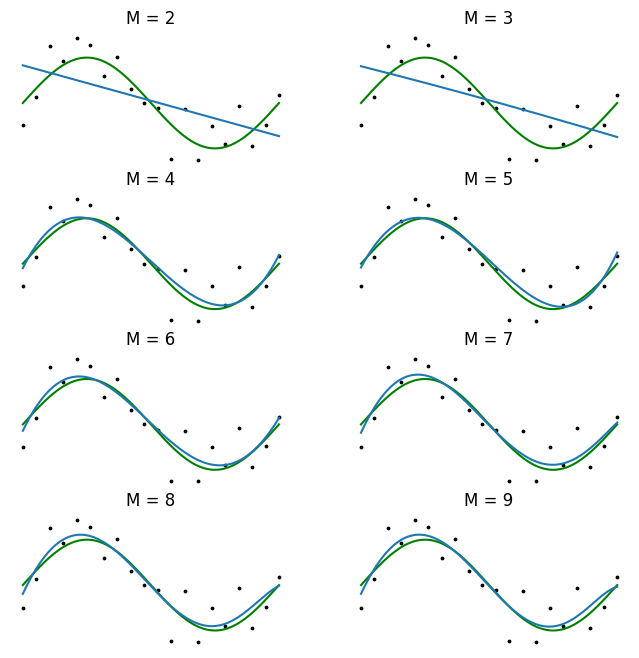
\includegraphics[width=5.20833in,height=\textheight]{./img/map_w.png}

}

\caption{Signal (green), training data (black), and fitted curves (blue)
for various settings of M -- the order of the polynomial, but with with
regularization governed by \(\text{ln } \lambda = 0\).}

\end{figure}



\end{document}
